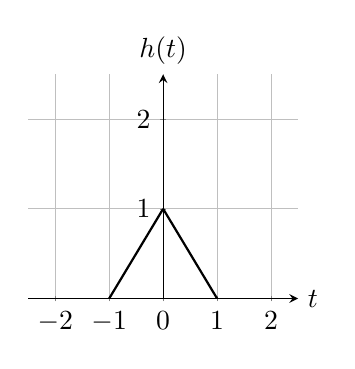
\begin{tikzpicture}
	\begin{axis}[
		xscale = 0.5,
		yscale = 0.5,
		xmin= -2.5, xmax = 2.5,
		ymin= 0, ymax = 2.5,
		axis x line=bottom,
		axis y line=center,
		xtick = {-2,-1,0,1,2},
		ytick = {1, 2},
		xlabel=$t$, xlabel style={at={(ticklabel* cs:1)}, anchor= west},
		ylabel=$h(t)$, ylabel style={at={(ticklabel* cs:1)}, anchor=south},
		grid=both,
		]
		\addplot[domain=-1:0, thick] (\x, \x + 1);
		\addplot[domain=0:1, thick] (\x, -\x + 1);
        \end{axis}
\end{tikzpicture}